% Template for Carleton problem sets
% Author: Andrew Gainer-Dewar, 20131
\documentclass[twoside]{article}
\usepackage{ccpset}
\usepackage{graphicx, pdfpages}
\usepackage{fixltx2e}

% The Latin Modern font is a modernized replacement for the classic
% Computer Modern. Feel free to replace this with a different font package.
\usepackage{lmodern}

%\titleformat{\subsection}[runin]{}{}{}{}[]

\title{EE445L - Lab 11 Report}
\author{Kevin Gilbert\\ Gilberto Rodriguez}
\date{May 2, 2014}
\prof{Professor Bard}
\course{Lab: Monday/Wednesday 5-6:15}

\begin{document}
\raggedbottom
\maketitle{}

\section{Requirements Document}
\subsection{Overview}
\subsubsection{Objectives}
Our project will be centered around developing a board to form the basis of a teleoperated car. The primary goal is to develop an RC car that will communicate wirelessly with a ZigBee and use onboard sensors, such as sonars and accelerometer,  to allow a level of self-control.
\subsubsection{Roles and Responsibilities}
This device is aimed towards DIY and hobbyist groups, as well as high school and college level robotics teams. Gilbert and I have designed the circuit schematic and software design layout as a group. PCB routing were handled primarily by a single person, as it is difficult to share work during this process. Soldering the componests to the board was handled by a single person at a time due to only having one borad and the danger of having two soldering irons in close proximity. Both of us tested individual components of the board to see basic functionality. We have handled any additional wiring/hardware modifications necessary. In case of an accidental shorting, we will find the necessary components to attepmt to fix our mistakes. The software realization was written by both of us as well. 
\subsubsection{Interactions with Existing Systems}
We will be using the LM3S1968 board as a controller for our device that will send commands through a ZigBee.
\subsection{Function Description}
\subsubsection{Functionality}
The system will have an on-board LM3S811 chip to collect data from the ZigBee and interface with the motors. Motor outputs are tied to onboard LEDs to help with debugging. The embedded device will also include motor controllers for actuation, and onboard sensors, such as sonars and accelerometer, to allow a degree of autonomity. The sonars and accelerometer are tied to capture pins on the 811 chip. There are two power regulators: a 3.3V regulator and a 5V regulator. The 3.3V regulator will be used to power the Xbee, LM3S811 chip, and accelerometer, and the 5V regulator will be used to power the sonar and motors. The Xbee is able to communicate bi-directionally using the API mode, so the two systems are able to communicate with each other. The 811 chip sends the sonar data to the 1968 to print ot the OLED.
\subsubsection{Performance}
The RC car has a range of approximately 40 meters thanks to the Xbee. ISR lengths were kept to a minimum. The sonars that we used contiously gave us random data on the 811 board. Overall, the RC car has a low current draw (under 1A). During testing, we were able to run the system fine during a 4-5 day timespan, so the system could theortically run for 1-2 days continuously (not advisable due to regulator heating concerns).
\subsubsection{Usability}
The LM3S1968 will be used to broadcast the wireless signal to the car. User input will be captured using a PSP joystick and a switch that will change between remote controlled and autonomous modes, and the car's speed will displayed on the onboard OLED. Currently, the RC car is able to send sonar data through the Xbee and receive motor commands for the 1968 from the Xbee. The motors are using PWM signals to run, and the sonars are tied to capture pins but are using GPIO based interrputs during a peroid of testing to check the differences between the sonar data. The RC car works fine as long as there is no XBee interference. Interference will cause either the Xbees to not initilize or stop receiving data. There is a switch on the controller, which will switch from teleoperated mode and autonomous. The switch functions correctly but autonomous mode is not currently implemented because of the lack of reliable sonar data.
\subsection{Deliverables}
\subsubsection{Reports}
We will write a report for Labs 11.
\subsubsection{Outcomes}

\noindent \bf{Lab11:}
\begin{enumerate}
\item Objectives: 2-page requirements document
\item Hardware Design :Detailed circuit diagram of the system (from Lab 7)
\item Software Design (no software printout in the report): Briefly explain how your software works (1/2 page maximum)
\item Measurement Data: As appropriate for your system. Explain how the data was collected.
\item Analysis and Discussion (1 page maximum) 
\end{enumerate}

\section{Hardware Design}
	\subsection{Circuit Schematics}
		\subsubsection{Control Circuit}
			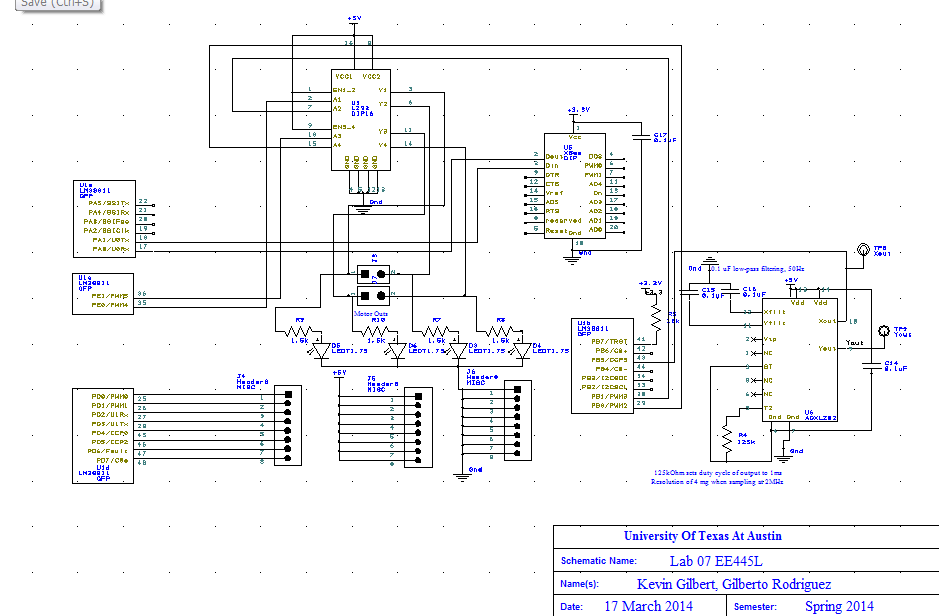
\includegraphics[width=\textwidth]{circuitDiagram}
		\subsubsection{Power Circuit}
			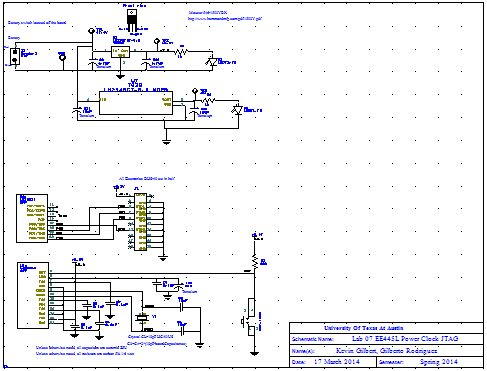
\includegraphics[width=\textwidth]{powerCircuit}

            
\section{Software Design}
Duplex communication between the XBees was implemented using API mode. The controller and car run in a stepped lock synchronized cycle. When the car receives a frame from the controller, the message string is parsed and the command executed (speed and direction of motors, and autonomous or teleoperated mode). The car would also trigger the sonars and measure the resulting distance. When primary functions were executed, the sonar and accelerometer data was packaged into a frame and transmitted back to the controller where the data would be graphed and displayed. \\ 

The hardware PWM on the LM3S811 ran into configuration issues with the timers being used for capture analysis, so they were dropped in lieu of software generated PWM. This was achieved through two periodic half-timer interrupt handlers that would reset their load values depending on the current state of the output pins. Four PWM signals were required for our half H-bridge circuit to implemented as a full H-bridge. Boolean flags were triggered in our main loop dependent on the incoming command packets from the controller, and used to switch direction in the handlers. The other four half timers were configured as edge triggered capture timers for the two sonars and each axis of the accelerometer. \\ 

Software design was kept as modular as possible to facilitate testing across embedded platforms. The autonomous design was focused towards obstacle avoidance given distance values from the sonars. Speed was also lowered through PWM to allow for easier avoidance due to the latency of the sonar sensors and shallow turn radius of our rack and pinion steering system. Accelerometer was confirmed to work in hardware, but the software still needs to be configured to avoid fractional calculation. The current design compares the time the signal is high to period, resulting in a percent which is not supported in hardware on the LM3S811 (or LM3S systems in general). The LM4F systems would be able to circemnavigate this problem. The lack of hardware PWM on the launchapds would also not be a problem as we are running it in software regardless.

\section{Measurement Data}
Estimated Current: 600 mA \\
Estimated Cost: \$34.70 for parts + \$53.00 for board (including shipping) = \$87.70 \\
\$20.00 overall (with free samples)

\section{Analysis and Discussion}
Most of the components of the board was in a working condition. We did have some trouble with getting the hardware PWM pins on the 811 working. The sonar module was developed on the LM3S1968 system and worked properly. When ported to the LM3S811 embedded system we designed, signals were read by our software from the sonar, but the distance readings were . We also had to completely rebuild the power circuit because we accidentily shorted the 5V regulator with the battery pins, which put us back an entire day since it blew the battery traces. Our new power circuit would cause our board to brown out whenever we tried to run the motors, so we had to try to get PWM working (we managed it in software since hardware PWM was still not functioning properly). There was an odd issue where the 3.3V regulator was heating up significantly even though the only thing it was powering was the 811, a LED, the accelerometer, and the Xbee. We are still unsure of the cause. We would have liked to do more testing with the accelerometer, but our major focus went to attempting to get a working PWM and sonar data. Not having working sonar data put a pause to some of our other plans, and we would like to figure out why the code was not porting correctly. Overall, it was a good learning experience to design and test our board as we now have a better understanding of the process, and our board was able to flash successfully, which was an awesome feeling. Ideally, we would go through a few design iterations in order to have a better power circuit and better optimize the space to prevent future shorts. 
 
\end{document}